\documentclass[letterpaper,11pt]{article}
% Soporte para los acentos.
\usepackage[utf8x]{inputenc}
\usepackage[T1]{fontenc}    
% Idioma español.
\usepackage[spanish,mexico, es-tabla]{babel}
% Soporte de símbolos adicionales (matemáticas)
\usepackage{multirow}
\usepackage{amsmath}		
\usepackage{amssymb}		
\usepackage{amsthm}
\usepackage{amsfonts}
\usepackage{latexsym}
\usepackage{enumerate}
\usepackage{ragged2e}
% Soporte para la imágenes.
\usepackage{graphicx}
% Modificamos los márgenes del documento.
\usepackage[lmargin=2cm,rmargin=2cm,top=2cm,bottom=2cm]{geometry}

\title{Universidad Nacional Autónoma de México \\
       Facultad de Ciencias \\
       Estructuras Discretas \\ 
       Tarea 2}
\author{Rubí Rojas Tania Michelle \\
        taniarubi@ciencias.unam.mx \\
        \# cuenta: 315121719}
\date{2 de octubre de 2017}

\begin{document}
\maketitle

\begin{enumerate}
    % Ejercicio 1.
    \item Sean $f^{(1)}, g^{(2)}$ símbolos de función, $P^{(1)}$ símbolo de 
    predicado. Clasifica las siguientes fórmulas como términos, fórmulas
    atómicas, fórmulas cuantificadas (con cuantificadores pero con presencias
    de variables libres) o enunciados (fórmulas con cuantificadores sin 
    variables libres); según el caso, justifica tu respuesta.

    \begin{itemize}
        % Ejercicio 1.1
        \item[a)] $f(g(a,b))$

        \textsc{Solución:} Es un término. Como las constantes $a$ y $b$ son 
        términos, entonces $g(a,b)$ también es un término ya que es un símbolo 
        de función aplicado a términos. 

        % Ejercicio 1.2
        \item[b)] $\neg ∀x ∀y (P(f(x)) \land Q(x, y))$

        \textsc{Solución:} Es un enunciado, ya que es una fórmula cuantificada 
        sin variables libres.

        % Ejercicio 1.3
        \item[c)] $P(g(f(x), y))$

        \textsc{Solución:} Es una fórmula atómica, ya que es un símbolo de  
        predicado aplicado a un término.

        % Ejercicio 1.4
        \item[d)] $∃x ∀y ∃z (R(x, y, z) \land Q(x, f(y)) → P(g(x,y)))$

        \textsc{Solución:} Es un enunciado, ya que es una fórmula cuantificada 
        sin variables libres.

        % Ejercicio 1.5
        \item[e)] $∀x ∀y ∀z (P(x, y) \land R(y, z)) \lor ∃z (Q(x, y, z))$

        \textsc{Solución:} Es una fórmula cuantificada, ya que las variables 
        $x$ y $y$ aparecen como variables libres en la fórmula $∃z (Q(x, y, z))$.
    \end{itemize}

    % Ejercicio 2.
    \item Traduce los siguientes enunciados a lógica de predicados. Indica de  
    manera clara la traducción de los predicados que utilizarás y el Universo
    de discurso.

    \textsc{Solución:} El Universo del discurso serán todas las personas,
    mientras que los predicados a utilizar son 

    \begin{itemize}
        \item $V(x):$ $x$ es voluntario.
        \item $A(x, y):$ $x$ ayuda a $y$.
        \item $M(x):$ $x$ es mexicano.
        \item $L(x):$ $x$ es militar.
        \item $J(x):$ $x$ es japonés.
        \item $N(x):$ $x$ es alemán.
    \end{itemize}

    Además, usaremos la constante $a:$ Armando.

    \begin{itemize}
        % Ejercicio 2.1
        \item[a)] Todos los voluntarios ayudan a alguien.

        \textsc{Solución:} $∀x (V(x) → ∃y (A(x, y)))$

        % Ejercicio 2.2
        \item[b)] Armando puede ayudar únicamente a un mexicano.

        \textsc{Solución:} $∀x ∀y (M(x) \land M(y) \land A(a, x) \land A(a, y) → x = y)$

        % Ejercicio 2.3
        \item[c)] Ningún militar puede ayudar a todas las personas.

        \textsc{Solución:} $∀x (L(x) → ∃y (\neg A(x, y)))$

        % Ejercicio 2.4
        \item[d)] Hay un mexicano al que todos los militares y japoneses lo 
        ayudan.

        \textsc{Solución:} $∃x ∀y (M(x) \land (L(y) \land J(y) → A(y, x)))$
        
        % Ejercicio 2.5
        \item[e)] Algún mexicano ayuda a todos o a nadie.

        \textsc{Solución:} $∃x (M(x) \land (∀y (A(x, y)) \lor ∀z (\neg A(x, z))))$

        % Ejercicio 2.6
        \item[f)] Hay algún mexicano que no puede ser ayudado por algún 
        japonés. 

        \textsc{Solución:} $∃x ∃y (M(x) \land J(y) \land \neg A(y, x))$
        
        % Ejercicio 2.7
        \item[g)] Algunos alemanes sólo ayudan a mexicanos.

        \textsc{Solución:} $∃x ∀y (N(x) \land (A(x, y) → M(y)))$

        % Ejercicio 2.8
        \item[h)] Exactamente una persona ayuda a todos menos a sí misma.

        \textsc{Sol.:} $∃x (\neg A(x, x) \land ∀y (x \neq y → A(x,y)) \land 
        ∀w (\neg A(w, w) \land ∀z (w \neq z → A(w,z))) → x = w)$

        % Ejercicio 2.9
        \item[i)] Exactamente una persona sólo se ayuda a sí misma.

        \textsc{Sol.:} $∃x (A(x, x) \land ∀y (x \neq y → \neg A(x, y)) \land 
        ∀w(A(w, w) \land ∀z(w \neq z → \neg A(w, x))) → x = w)$

        % Ejercicio 2.10
        \item[j)] Algunos militares no ayudan a los mexicanos.

        \textsc{Solución:} $∃x ∀y (L(x) \land (M(y) → \neg A(x, y)))$

        % Ejercicio 2.11
        \item[k)] Todos los voluntarios japoneses ayudan a algún mexicano. 

        \textsc{Solución:} $∀x (V(x) \land J(x) → ∃y (M(y) \land A(x, y)))$

        % Ejercicio 2.12
        \item[l)] Armando ayuda a los mexicanos, por lo tanto los voluntarios
        Ayudarán a los mexicanos. 

        \textsc{Solución:} $∀x (M(x) → A(a, x)) → ∀y ∀z (V(y) \land 
        M(z) → A(y, z))$
    \end{itemize}

    % Ejercicio 3.
    \item Considera los siguientes predicados 

    \begin{itemize}
        \item $P(x):$ $x$ es un número par.
        \item $M(x, y):$ $x$ es menor que $y$.
        \item $G(x, y):$ la división de $x$ entre $y$ está dentro del conjunto.
    \end{itemize}

    Y los siguientes enunciados

    \begin{itemize}
        \item $∀x ∀y (M(x, y) → ∃z(M(x, z) \land M(z, y)))$
        \item $∀x (P(x) → M(0, x))$
        \item $∀x ∀y (x \neq 0 \land y \neq 0 → (G(x, y) \land G(y, x)))$
        \item La negación del inciso $c)$         
    \end{itemize}

    \newpage
    Evalúa su valor de verdad con respecto a los siguientes Universos del 
    discurso. Para aquellos enunciados que sean falsos, exhibe un 
    contraejemplo.

    \begin{itemize}
        % Ejercicio 3.1
        \item[a)] Los números naturales (el $0$ también es natural).

        \textsc{Solución:}
        \begin{itemize}
            \item $∀x ∀y (M(x, y) → ∃z(M(x, z) \land M(z, y)))$

            El enunciado evalúa a falso. Si tomamos $x = 1$ y $y = 2$, entonces 
            notamos que en los números naturales, no hay un número entre el $1$
            y el $2$. 

            \item $∀x (P(x) → M(0, x))$

            El enunciado evalúa a verdadero. En los números naturales, 
            cualquier número par es mayor que el $0$.

            \item $∀x ∀y (x \neq 0 \land y \neq 0 → (G(x, y) \land G(y, x)))$

            El enunciado evalúa a falso. Si tomamos $x = 1$ y $y = 2$ entonces 
            tenemos que $\frac{1}{2} = 0.5$ y éste no pertence al conjunto de 
            los naturales. 

            \item La negación del inciso $c)$
            
            El enunciado evalúa a verdadero. Se afirma que existen dos números 
            naturales $x$ y $y$ tales que son diferente de cero y la división
            $\frac{x}{y}$ o $\frac{y}{x}$ se encuentra dentro del conjunto;
            así, como sabemos que si tomamos $x = 1$ y $y = 2$ entonces 
            $\frac{2}{1}$ se encuentra dentro del conjunto. 
        \end{itemize}

        % Ejercicio 3.2
        \item[b)] Los números reales.

        \textsc{Solución:}
        \begin{itemize}
            \item $∀x ∀y (M(x, y) → ∃z(M(x, z) \land M(z, y)))$

            El enunciado evalúa a verdadero. Sabemos que hay una infinidad de  
            números entre cualesquiera dos números.

            \item $∀x (P(x) → M(0, x))$

            El enunciado evalúa a falso. En los números reales, hay una infinidad 
            de números pares que son menores al $0$.

            \item $∀x ∀y (x \neq 0 \land y \neq 0 → (G(x, y) \land G(y, x)))$

            El enunciado evalúa a verdadero. En los números reales, para 
            cualesquiera dos números $x$ y $y$, las divisiones $\frac{x}{y}$ y 
            $\frac{y}{x}$ se encuentran dentro del conjunto. 

            \item La negación del inciso $c)$     
            
            El enunciado evalúa a falso, ya que el inciso anterior evalúa a 
            verdadero.
        \end{itemize}

        % Ejercicio 3.3
        \item[c)] Los números enteros. 

        \textsc{Solución:}
        \begin{itemize}
            \item $∀x ∀y (M(x, y) → ∃z(M(x, z) \land M(z, y)))$

            El enunciado evalúa a falso. Si tomamos $x = 1$ y $y = 2$, entonces 
            notamos que en los números naturales, no hay un número entre el $1$
            y el $2$. 

            \item $∀x (P(x) → M(0, x))$

            El enunciado evalúa a falso. En los números enteros, hay una 
            infinidad de números pares que son menores al $0$.

            \item $∀x ∀y (x \neq 0 \land y \neq 0 → (G(x, y) \land G(y, x)))$

            El enunciado evalúa a falso. Si tomamos $x = 1$ y $y = 2$, entonces 
            tenemos que $\frac{1}{2} = 0.5$ no se encuentra dentro del conjunto.

            \item La negación del inciso $c)$   
            El enunciado evalúa a verdadero. Se afirma que existen dos números 
            naturales $x$ y $y$ tales que son diferente de cero y la división
            $\frac{x}{y}$ o $\frac{y}{x}$ se encuentra dentro del conjunto;
            así, como sabemos que si tomamos $x = 1$ y $y = 2$ entonces 
            $\frac{2}{1}$ se encuentra dentro del conjunto.       
        \end{itemize}
    \end{itemize}

    % Ejercicio 4.
    \item El micromundo de figuras tiene los enunciados siguientes:

    \begin{itemize}
        \item $T(x), C(x)$ y $S(x)$ tales que $x$ es triángulo, cuadrado o 
        círculo, respectivamente.
        \item $P(x), M(x)$ y $G(x)$ tales que $x$ es pequeño, mediano o 
        grande, respectivamente.
        \item $Su(x, y), N(x, y), E(x, y)$ y $O(x, y)$ para indicar que $x$ 
        está al sur, norte, este u oeste de $y$, respectivamente.
        \item $Co(x, y)$ y $R(x, y)$ para indicar que $x$ está en la misma 
        columna o renglón que $y$, respectivamente.
    \end{itemize}

    Para cada una de las siguientes fórmulas, escribe su traducción al español,
    da un micromundo no vacío donde la fórmula sea verdad y uno donde sea 
    falsa.

    \begin{itemize}
        % Ejercicio 4.1
        \item[a)] $∃x ∃y ∃z (T(x) \land C(y) \land S(z) \land N(x, y) \land 
                  N(y,z))$

        \textsc{Solución:} Existe un triángulo, un cuadrado y un círculo tales 
        que el triángulo se encuentra al norte del cuadrado y el cuadrado se 
        encuentra al norte del círculo.

        % Ejercicio 4.2
        \item[b)] $∀x (S(x) → \neg G(x)) \land ∀x (C(x) → ∃y (Co(x, y) \land 
                  T(x) \land P(x)))$

        \textsc{Solución:} Cualquier círculo no es grande y para todo cuadrado  
        existe un triángulo pequeño que se encuentra en la misma columna.

        % Ejercicio 4.3
        \item[c)] $∀x ∃y (R(x, y) → (M(x) \lor G(y)))$ 

        \textsc{Solución:} Para cualquier figura $x$ existe otra figura $y$ tal 
        que si $x$ está en el mismo renglón que $y$, entonces $x$ es mediana 
        o $y$ es grande. 

        % Ejercicio 4.4
        \item[d)] $∃x (C(x) \land ∀y (N(y, x) → P(y) \lor S(y))) \land 
                  ∀w (C(w) → ∃y (G(y) \land E(y, w)))$

        \textsc{Solución:} Hay un cuadrado tal que para cualquier figura que se 
        encuentre al norte se tiene que esa figura es pequeña o es un círculo.
        Además, para cualquier cuadrado $w$ existe una figura grande que se 
        encuentra al este de $w$.
    \end{itemize}

    El siguiente micromundo modela a todas las fórmulas fórmulas cuando son 
    verdaderas:

    \begin{center}
        \centerline{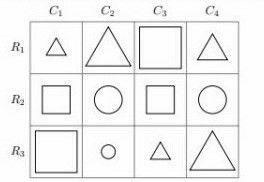
\includegraphics[scale=0.7]{modelo1.jpg}}
    \end{center}

    Y el siguiente micromundo modela a todas las fórmulas cuando son falsas:

    \begin{center}
        \centerline{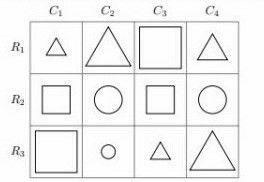
\includegraphics[scale=0.7]{modelo2.jpg}}
    \end{center}
\end{enumerate}

\end{document}
